\section{Echtzeitbetrieb}

\subsection{Kriterien}
\begin{itemize}
	\item \underline{Pünktlichkeit/Rechtzeitigkeit} (timeliness)
	\item \underline{Sicherheit} (Safety) (Fail-safe/Fail-Operational; Automotive, Luft/Raumfahrt)
	\item \underline{Verfügbarkeit}
	\item \underline{Deterministisch} (in gegebenem Zustand liefert das System bei gegebener Eingabe immer dieselbe Ausgabe)
\end{itemize}

\subsection{Klassifizierung: Echtzeitbedingung}
\begin{itemize}
	\item Hart \\
	\underline{muss} rechtzeitig/pünktlich ausgeführt werden
	
	\item Weich \\
	darf \underline{Toleranz} nicht überschreiten
	
	\item Fest \\
	\underline{sollte} rechtzeitig/pünktlich ausgeführt werden, sonst \underline{nutzlos}
\end{itemize}

\subsection{Laufzeit-Modell}
\begin{figure}[h!]
	\begin{center}
		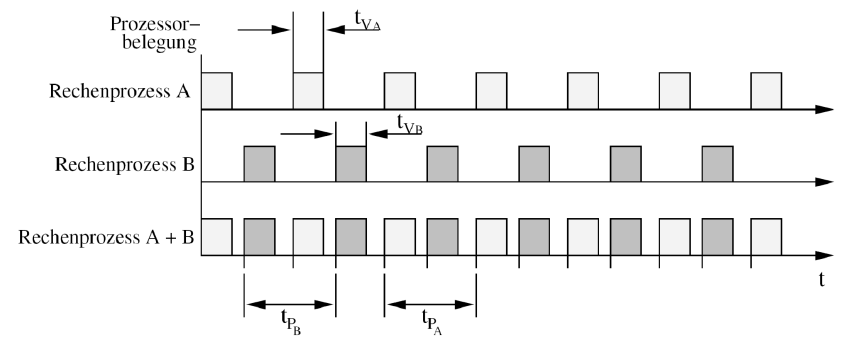
\includegraphics[width=.75\linewidth]{pics/laufzeit}
		\caption{Prozessauslastung}
	\end{center}
\end{figure}

\begin{itemize}
	\item Verarbeitungszeit: $t_v$
	\item Prozesszeit: $t_p$
	\item Auslastung: $\rho = \frac{t_v}{t_p}$
	\item Gesamtauslastung: $\rho_{ges} = \sum_{i=0}^{n}\frac{t_{v_i}}{t_{p_i}}$ (muss $\leq 1$ sein)
\end{itemize}

\subsection{Pünklich vs Rechtzeitig}
\begin{figure}[h!]
	\begin{center}
		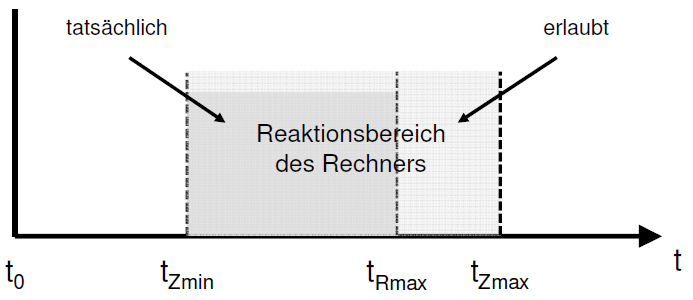
\includegraphics[width=.75\linewidth]{pics/puenktlichkeit}
		\caption{Echtzeitbedingung: Pünktlichkeit}
	\end{center}
\end{figure}
\begin{itemize}
	\item Wartezeit: $t_w$
	\item Reaktionszeit: $t_R = t_v + t_w$
	\item Zulässigkeit: $t_{Z_{min}}$, $t_{Z_{max}}$
	\begin{itemize}
		\item Pünktlich: $t_{Z_{min}} \leq t_{R_{min}} \leq t_R \leq t_{R_{max}} \leq t_{Z_{max}}$
		\item Rechtzeitig: $t_R \leq t_{R_{max}} \leq t_{Z_{max}}$
	\end{itemize}
\end{itemize}